Bio2BEL comprises numerous independent open-source Python packages that each enable reproducible access to a given biological data source (Figure 1).
Each Bio2BEL package contains five components: 1) a definition of the source database or knowledge base, 2) an automated downloader for the data, 3) a parser for the data, 4) a storage and querying system for the data, and 5) a protocol for serializing the data to BEL (Figure 2).
In this section, we outline the components of a Bio2BEL package and their implementation details.

\begin{figure}
    %\captionsetup{format=plain}
    \makebox[\textwidth]{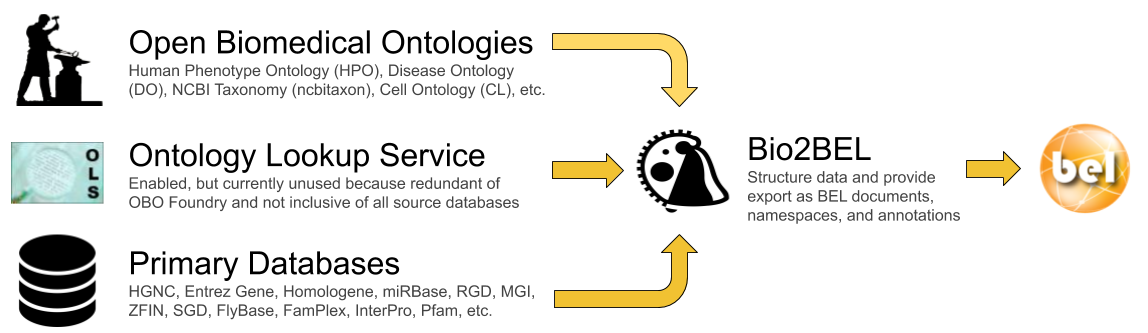
\includegraphics[width=120mm]{figures/schema.png}}
    \caption[Schema of Bio2BEL]{Though their main focus is on generating BEL documents, some Bio2BEL repositories have secondary goals of generating the BEL namespace and annotation files necessary to support manual curation. Most rely on primary databases, but the Bio2BEL framework also includes functions for generating them from standard Open Biomedical Ontology documents, or through the EBI Ontology Lookup Service~\cite{Cote2006a}. Logos adapted from \url{http://obofoundry.org}, \url{https://www.ebi.ac.uk/ols}, and \url{https://openbel.org}.}
    \label{fig:schema}
\end{figure}


\subsection*{Components of a Bio2BEL package}

As this section outlines the core components and philosophy of a Bio2BEL package, it illustrates the tasks and thought process of a scientific software developer as they implement a new Bio2BEL package.

\begin{figure}
    %\captionsetup{format=plain}
    \makebox[\textwidth]{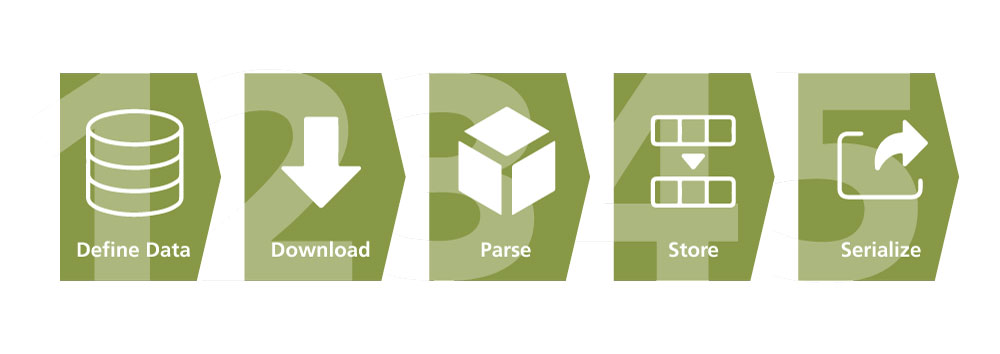
\includegraphics[width=120mm]{figures/components.jpg}}
    \caption[Components of Bio2BEL]{A graphical overview of the sequentially ordered components of a Bio2BEL package. These components correspond to the philosophy that reproducibility and accessibility can ultimately lead to the democratization of the usage of prior biological knowledge.}
    \label{fig:components}
\end{figure}

\subsubsection*{Definition of data}

The first step in generating a Bio2BEL package is to understand the source data.
This requires determining if the data are publicly accessible, if they are versioned (and how the location changes with versions), and if they are available under a permissive license.
Bio2BEL packages do not contain data themselves and only refer to the locations of the original data sources.
For those that are versioned, providers commonly generate symlinks to the most recent version (e.g., InterPro; \url{ftp://ftp.ebi.ac.uk/pub/databases/interpro}).
These characteristics help minimize licensing issues while enabling the resulting packages to update their content without changing code.
Then, the developer implements custom code that makes the appropriate interpretations to convert the source data to BEL.
Below, three types of data that can be readily integrated in BEL are described along with accompanying Table~\ref{tab:statements}.

\begin{table}[h!]
\caption{Example BEL statements generated by several different types of data sources}
\label{tab:statements}
\begin{tabular}{llll}
\hline
  Data Source Type
  & Data Source            & Example BEL Statement                     & Description \\
\hline
\multirow{3}{*}{Taxonomies, Hierarchies, and Ontologies}
  & MeSH                   & path(X) isA path(Y)                       & Pathology X is a subtype of pathology Y. \\
  & Complex Portal         & p(X) partOf complex(Y)                    & Protein X is a member of complex Y. \\
  & GO                     & bp(X) partOf bp(Y)                        & Biological process X is a sub-process of Y. \\
\hline
\multirow{2}{*}{Tabular and Relational Data}
  & PubChem, ChEMBL        & a(X) directlyDecreases act(p(Y), ma(kin)) & Compound X inhibits kinase Y. \\
  & ADEPTUS                & path(X) positiveCorrelation r(Y)\newline
path(X) negativeCorrelation r(Y)\newline
path(X) causeNoChange r(Y)
& Gene Y has been observed to either be up-regulated, down-regulated, or unregulated in patients with pathology X. \\
\hline
Graphs
  & Menche \textit{et al.} & path(X) association path(Y)               & Pathology X is statistically similar to pathology Y on the basis of gene overlap as defined by Menche \textit{et al.}~\cite{Menche2015}. \\
\end{tabular}
\end{table}

\paragraph*{Taxonomies, hierarchies, and ontologies}

The Medical Subject Headings~\cite{ROGERS1963} multi-hierarchy can be converted to BEL by generating an isA relationship between each MeSH descriptor and all of its corresponding parents in the associated MeSH tree.
Nomenclatures like the Complex Portal~\cite{Meldal2015} also define partOf relations between protein complexes and their substituents.
The multi-hierarchy in Gene Ontology (GO~\cite{Carbon2017}) can be converted similarly, which contains both isA relations and partOf relations.

\paragraph*{Tabular and Relational Data}

Enzyme inhibitors from ChEMBL and PubChem can be encoded like a(X) directlyDecreases act(p(Y), ma(kin)), and disease-specific differential gene expression can be encoded like path(X) positiveCorrelation r(Y) or path(X) negativeCorrelation r(Y), or path(X) causeNoChange r(Y) depending on whether the gene's expression is up-regulated, down-regulated, or not regulated, respectively.
Further, BEL relationships can be extended include metadata (i.e., annotations) describing their quantitative aspects.
For example, $IC_{50}$, $EC_{50}$, or other kinetic assay measurements as well as provenance and biological contextual information (e.g., original publication, cell line, assay type) can be included with the enzyme inhibition relationships from ChEMBL\@.
Similarly, the $log_2$$ fold change and $p$-values can be included with relationships about differential gene expression.

\paragraph*{Graphs}
Wet-laboratory experimentation can be used to generate networks of directly observed phenomena (e.g., protein-protein interaction networks) and indirectly observed phenomena (e.g., gene co-expression networks).
Graphs are often distributed as tabular data to include additional information about their constituent nodes and edges and there is often overlap with the previous data type describing tabular and relational data.
\textit{In silico} experimentation can also be used to derive edges from experimental data sets or even other graphs.
For instance, bipartite graphs can be projected to homogeneous graphs consisting of a single entity and edge type as suggested by Sun \textit{et al.}~\cite{Sun2014}.
Menche \textit{et al.}~\cite{Menche2015} used this strategy and computed a homogenous graph of disease-disease associations from a bipartite graph of diseases and their associated genes.

\subsubsection*{Downloader}
The Bio2BEL framework follows a functional programming paradigm to provide an abstraction of the acquisition of data over common internet protocols like HTTP, HTTPS, and FTP\@.
With only the URL of the data set as an input, Bio2BEL generates a download function that wraps Python's built-in urllib module and a simple caching mechanism in the local filesystem that avoids unnecessary network usage and duplication of potentially large files.
However, some data sources, such as DrugBank~\cite{Wishart2018}, are not available without authentication and cannot make use of this abstraction. In those cases, developers can substitute the standard code provided in the Bio2BEL framework with custom implementations.
We have taken this route for several of the packages presented in the Results section of this paper for repositories including DrugBank and MSigDB~\cite{Liberzon2015}.

\subsubsection*{Parser}
There are several common file formats used by biological data sources (e.g., CSV, TSV, XML, RDF, JSON, KGML, Stockholm, OBO, OWL).
Data may also (and sometimes only) be accessible through public application programming interfaces (APIs) such as the data from KEGG~\cite{Kanehisa2017}, Reactome~\cite{Fabregat2018}, and BioThings~\cite{Xin2016}.
Alternatively, data may be available through software packages usage such the Affymetrix R package~\cite{Gautier2004} and HaploReg (Ward and Kellis, 2012).
After each Bio2BEL package's downloader generates a local copy of the data, the developer can either use one of the pre-defined parser functions from the Bio2BEL framework or implement a custom parser.
For the most simple formats (i.e., CSV and TSV), the Bio2BEL framework automatically generates a parser that uses the pandas package (McKinney, 2010; \url{https://github.com/pandas-dev/pandas}).
Formats like XML, JSON, and Stockholm have corresponding parsers built into the Python language or standard biology-focused packages, but the information contained within often needs custom logic for restructuring such as in the case of KGML, BioPAX, or PSI MI-XML.
The remaining custom formats all require custom parsers and logic.
We have already implemented Bio2BEL that used CSV and TSV data (e.g., InterPro, ExCAPE-DB), XML (e.g., DrugBank), RDF (e.g., WikiPathways), JSON and KGML (e.g., KEGG), Stockholm (e.g., miRBase), and OBO and OWL (e.g., GO, DOID).

In the case of tabular data, the developer has the opportunity to annotate the column headers and their corresponding data types, which are not always included in the data and may be sought from various readme files or by exploring the corresponding website.
Further, the contained data might be more useful after normalization or augmentation with information from other biological data sources.
Because some databases provide identifiers with redundant information, such as the duplication of the namespace in the identifier, they must be normalized.
For example, each identifier in the Disease Ontology (Schriml et al., 2018) is prefixed by its namespace, DOID, as can be seen in the Compact URI for the entry for restless legs syndrome, DOID:DOID:0050425.
In the corresponding Bio2BEL DOID package, as well as those for others (e.g., HGNC, Gene Ontology) we normalized these identifiers to remove the redundant information.
Because the main Entrez Gene database does not contain crucial information for genes, such as their chromosomal coordinates in various genomic builds, we augmented the data in the Bio2BEL Entrez package for each gene with information from RefSeq so that the genomic positions and corresponding genome build for each gene were readily accessible.
Additionally, several databases that reference genes only use their HGNC gene symbols and not stable identifiers, and therefore require this additional normalization step.

\subsubsection*{Storage}
Though this step may be considered optional after parsing the data, it is helpful for future reuse to choose a database type and develop a schema with which the data can be stored.
Often, relational databases that can be queried with SQL are an appropriate choice.
The Bio2BEL framework provides a full harness for generating an object-relational mapping (ORM) using the SQLAlchemy (\url{https://www.sqlalchemy.org}) Python package that handles generation of the SQL schema and storage of the data in a SQL database.
Corresponding entity-relation diagrams can be found in the supplementary data repository at \url{https://github.com/bio2bel/bio2bel-manuscript-supplement}.
While all Bio2BEL packages have, until now, used SQL databases with the SQLAlchemy ORM, there exists alternatives such as graph databases built on RDF or property graphs like Neo4J or OrientDB with a corresponding object-graph mapper that have been successfully employed in downstream applications using biological knowledge graphs (Himmelstein et al., 2017; Saqi et al., 2018).

\subsubsection*{Serializer}
The final aspect of a Bio2BEL package is either to serialize the parsed data as BEL or to export the accompanying database as BEL. Entities in the SQL database that correspond to nodes and edges in BEL graphs can be converted by extending their respective ORM classes with Python functions using the internal domain-specific language provided by PyBEL (Hoyt et al., 2018a).
It can then be output in several formats provided by PyBEL and its growing ecosystem of plugins as well as it shields Bio2BEL packages from changes to the BEL language.
Additionally, some Bio2BEL packages wrap standard nomenclature resources such as HGNC (Yates et al., 2017) and are able to generate BEL namespace files that are a necessary in both manual and automated curation of content in BEL (Figure 2).
This step is deeply connected with the prior step related to the definition of the data.

\subsection*{Implementation Details}
The Bio2BEL framework and Bio2BEL packages are implemented in Python with accessibility and readability in mind.
The framework provides an abstract class bio2bel.Manager whose functionality all Bio2BEL packages must completely implement.
Using these definitions, the framework automatically generates a uniform command line interface (CLI) that includes functions for populating the database, clearing the database, reloading data from the source, generating a web application with a view over the contents of the database, and serializing to BEL\@.

The Bio2BEL framework and Bio2BEL packages use flake8 (\url{https://github.com/PyCQA/flake8}) to enforce code quality, a setup.cfg file to describe the package, setuptools (\url{https://github.com/pypa/setuptools}) to build distributions, pyroma (\url{https://github.com/regebro/pyroma}) to enforce package metadata standards, sphinx (\url{https://github.com/sphinx-doc/sphinx}) to build documentation, Read the Docs (\url{https://readthedocs.org}) to host documentation, pytest (\url{https://github.com/pytest-dev/pytest}) as a testing framework, coverage (\url{https://github.com/nedbat/coveragepy}) and Codecov (\url{https://codecov.io}) to monitor testing coverage, and Travis-CI (\url{https://travis-ci.com}) as a continuous integration service.
Further, we provide a template for Cookiecutter (\url{https://github.com/audreyr/cookiecutter}) at \url{https://github.com/bio2bel/bio2bel-cookiecutter} such that the structure of new packages can be quickly generated containing all of the configuration for each of these tools.

\subsection*{Implications of the Bio2BEL Philosophy}
Because all Bio2BEL packages are uniform in their implementation and CLI usage, it is trivial to provide a Dockerfile and Docker-Compose configuration for quick deployments.
In the future, we plan to automatically generate RESTful APIs, which may be more useful to deploy internally than to use publicly available ones due to constraints like rate-limits.
Because all Bio2BEL packages are independent, they avoid two major problems of monolithic codebases: they are more robust to breakages or failures in a single package and they can be installed as needed, which is pertinent as the data sources become larger, more heterogeneous, and more complex.

Further, Bio2BEL packages can be generated by any group, and registered with the Bio2BEL framework using Python entry points (\url{https://packaging.python.org/specifications/entry-points}) that can be defined in the installation configuration.
While the Cookiecutter template allows new developers to quickly generate a package with the correct format, a full tutorial for implementing a uniform Bio2BEL package can be found at \url{https://bio2bel.readthedocs.io/en/latest/tutorial.html}.

